
\RequirePackage{fix-cm}
%
%\documentclass{svjour3}                     % onecolumn (standard format)
%\documentclass[smallcondensed]{svjour3}     % onecolumn (ditto)
%\documentclass[smallextended]{svjour3}       % onecolumn (second format)
\documentclass[twocolumn]{svjour3}          % twocolumn
%
\smartqed  % flush right qed marks, e.g. at end of proof
%
\usepackage{graphicx}
%
% \usepackage{mathptmx}      % use Times fonts if available on your TeX system
%
% insert here the call for the packages your document requires
%\usepackage{latexsym}
% etc.
%
\usepackage{amsfonts,amssymb,amsmath,
            amssymb,amsopn,amsxtra,amstext,amsbsy}
\usepackage{epsfig}
\usepackage[makeroom]{cancel}
\usepackage{array,arydshln}
\usepackage{array}
\usepackage{url}
%\usepackage{tikz}
\usepackage[utf8x]{inputenc}
\usepackage{fancyhdr}
\usepackage{hyperref,wasysym}
\usepackage{color}
\usepackage{enumerate}
\usepackage{algorithm}
\usepackage{algorithmic}
\renewcommand{\algorithmicrequire}{\textbf{Input:}}
\renewcommand{\algorithmicensure}{\textbf{Output:}}
\usepackage{multirow}
%\usepackage[spanish]{babel}

%%%%%%%%%%%%%%%%%%%%%%%%%%%%%%%%%%%%%%%%%%%%%%%%%%%%%%%%%%%%%%%%%%%%%%%%%%%%%%%%%%%%%%%%%%%
\usepackage{xcolor}%%%%%%%%%%%%%%%%%%%%%%%%%%%%%%%%%%%%%%%%%%%%
\usepackage{hyperref}%%%%%%%%%%%%%%%%%%%%%%%%%%%%%%%%%%%%%%%%%%
\usepackage{pmat}%%%%%%%%%%%%%%%%%%%%%%%%%%%%%%%%%%%%%%%%%%

%\newtheorem*{myteo}{Teorema}
%\newtheorem*{mydef}{Definici\'on}
%% MYREMARK ENVIRONMENT %%%%%%%%%%%
\newenvironment{mycolor}{\color{blue}}{}
\newcounter{myremarkcount}
\setcounter{myremarkcount}{0}
\newsavebox{\myremarkbox}
\newenvironment{myremark}
{% This is the begin code
\medskip
\begin{flushright}
\begin{lrbox}{\myremarkbox}%
\begin{minipage}[t]{1.00\linewidth}
\stepcounter{myremarkcount}
\footnotesize
\begin{mycolor}
{{\bf Proofreading Remark.}\ }
% \begin{it}
}
{% This is the end code
% \end{it}
\end{mycolor}
\end{minipage}
\end{lrbox}
\fbox{\usebox{\myremarkbox}}
\end{flushright}

\bigskip}

%%%%%%%%%%%%%%%%%%%%%%%%%%%%%%%%%%%%%%%%%%%%%%%%%%%%%%%%%%%%%%%%%%%%%%%%%%%%%%%%%%%%%%%%%%%


\journalname{Applied Intelligence}


\begin{document}

\title{Intraday Forex rates forecasting using an online cointegration approach}
%\subtitle{Do you have a subtitle?\\ If so, write it here}

%\titlerunning{Short form of title}        % if too long for running head

\author{Paola Arce \and Werner Kristjanpoller \and Luis Salinas }

%\authorrunning{Short form of author list} % if too long for running head

\institute{P. Arce  \at
              Departamento de Inform\'atica, Universidad T\'ecnica Federico Santa
              Mar\'ia\\
              Tel.: +56-32-2654000\\
              %Fax: +123-45-678910\\
              \email{paola.arce@usm.cl}           %  \\
%             \emph{Present address:} of F. Author  %  if needed
           \and
           W. Kristjanpoller \at
              Departamento de Industrias, Universidad T\'ecnica Federico Santa
              Mar\'ia\\
              %Fax: +123-45-678910\\
              \email{werner.kristjanpoller@usm.cl}             \\
           \and
           L. Salinas \at
              Departamento de Inform\'atica, Universidad T\'ecnica Federico Santa
              Mar\'ia\\
              Centro Científico Tecnológico de Valparaíso (CCTVal) \\
              \email{luis.salinas@usm.cl}           %  \\
}

\date{Received: date / Accepted: date}
% The correct dates will be entered by the editor


\maketitle

\begin{abstract}

%A Vector Error Correction Model (VECM) is an econometric model which
%characterizes the joint dynamic behaviour of a set of cointegrated variables. It
%is said that two non-stationary time series are cointegrated if a linear
%combination of them exhibit a stationary behaviour. 
%
%Cointegration is commonly found in finance and it has been shown that
%introducing cointegration restrictions often improves forecasting. However,
%determining VECM parameters and how much of the historical data is useful for
%making a forecast is a computational challenge.  
%
%In this study, we propose a new version of VECM whose parameters are obtained
%adaptively using parallel computing taking into account the cointegrated
%behaviour of the time series. The methodology is tested using data of the
%Foreign Exchange (Forex) market. Numerical experiments show that our adaptive
%and parallel approach significantly improves execution times with respect to the
%common serial processing and forecasts are made before new data arrives.  
Vector error correction model (VECM) parameters are commonly obtained using the
ordinary least squares method. Since this parameters could be sensitive to the
data, this proposal is to get these parameters using ridge regression which
could lead to a better generalization capability. In order to give with a
real-time response, an online version of VECM (OVECM) is proposed. OVECM solves
VECM considering only a sliding window of historical data and therefore
better response times could be achieved.


\keywords{VECM \and Cointegration \and Forex \and MPI \and Parallel algorithm}

\end{abstract}

\section{Introduction}
\label{sec:introduction}
VECM introduces the long-run relationship among a set of cointegrated variables
as an error correction term. VECM is a special case of the vector autorregresive
model (VAR) model. VAR model expresses future values as a linear combination of
variables past values.  However, VAR model cannot be used with non-stationary
variables, which is a common feature of financial assets. VECM is a linear model
but in terms of variable differences. If cointegration exists, variable
differences are stationary and they introduce an error correction term which
adjusts coefficients to bring the variables back to equilibrium. In finance,
many economic time series turn to be stationary when they are differentiated and
cointegration restrictions often improves forecasting~\cite{duy1998}. Therefore,
VECM has been widely adopted.

Both VECM and VAR model parameters are obtained using ordinary least squares
(OLS) method. OLS has two main problems: is sensitive to errors on input data
and involves many calculations. The former problem is commonly solved using
Ridge Regression (RR) \cite{hoerl1970} which introduces a regularization
parameter that leads to an unbiased estimation with better generalization
capability. The second problem of computational complexity depends on the number
of past values and observations considered.  Recently, online learning
algorithms have been proposed to solve problems with large data sets because of
their simplicity and their ability to update the model when new data is
available. 

Our proposal is an online formulation of the VECM called Online VECM (OVECM)
based on consideration of only a sliding window of the historical data.  OVECM
introduces matrix optimizations in order to reduce the number of operations and
also takes into account the fact that cointegration vector space doesn't
experience large changes with small changes in the input data. Moreover, OVECM
uses RR instead of OLS to obtain VECM parameters. Our method is later tested using four
currency rates from the foreign exchange market with a frequency of 10 seconds.
Model effectiveness is focused on out-of-sample forecast rather than in-sample
fitting.  This criteria allows the OVECM prediction capability to be expressed
rather than just explaining data history. Our method performance is compared
with its optimal offline algorithm.

\section{Background}
\label{sec:background}
\subsection{Integration and Cointegration}\label{sec:coint}\  
Following Johansen \cite{johansen1995} we shall say that a stochastic process
$Y_t$ which satisfies $Y_t-E(Y_t) = \sum_{i=0}^\infty C_i\,\varepsilon_{t-i}$ is
called $I(0)$, and then we shall write $Y_t\sim I(0)$, whenever
$\sum_{i=0}^\infty C_i \neq 0$ and $\sum_{i=0}^\infty C_i\,z^i$ converges for
$z\in\mathbb{C}$ with $|z|<1$.  It is understood that the condition
$\varepsilon_t\sim iid(0,\sigma^2)$ holds.

A (vector) time series $\mathbf{y}_t$ is said to be {\em integrated of order\/}
$d$, and then we shall write $\mathbf{y}_t\sim I(d)$, whenever after $d$ times
(discrete) differentiation an stationary process is obtained~\cite{banerjee1993};
more precisely, whenever
$(1-L)^d\,\mathbf{y}_t\sim\text{I(0)}$, where $L$ is the usual lag operator:
$(1-L)\,\mathbf{y}_t = \Delta\mathbf{y}_t = \mathbf{y}_t-\mathbf{y}_{t-1}$ for
all $t$.  

Note that this definition includes the scalar case as time series of
vectors of dimension 1; in this scalar case we will write the time series in
nonbold format.

Let $\mathbf{y}_t^\nu$, $\nu=1,\dots,p$, be a set of $p$ vector time series of
order $I(1)$.  They are said to be {\em cointegrated\/} if a vector
$\beta=[\beta(1),\dots,\beta(p)]^\top \in \mathbb{R}^p$ exists, such that the
time series,
\begin{equation}
\mathbf{Z}_t:= 
\sum_{\nu=1}^p \beta(\nu)\,\mathbf{y}_t^\nu\,\sim\,\text{I(0)}\,.
\end{equation}
In other words, a set of $I(1)$ time series is said to be cointegrated if a
linear combination of them exists, which is I(0).


\subsection{Vector Autorregresive Models}\label{sec:varvec}

VECM is a special case of VAR model and both describe the joint behaviour
of a set of variables.

The VAR($p$) model is a general framework describing the behaviour of a
set of $l$ endogenous variables as a linear combination of their last $p$
values, where $l,p\in\mathbb{N}$. 
In our case, each one of these $l$ variables is a scalar time series
$y_{\lambda,t}$, $\lambda=1,\dots,l$, and we represent them all together
at time $t$ by the the vector time series:
\begin{equation}
\label{eq:variables}
\mathbf{y}_t = 
\begin{bmatrix} y_{1,t} & y_{2,t} & \dots & y_{l,t} \end{bmatrix}^\top.
\end{equation}
\noindent
Notice that the vectors $\mathbf{y}_t$ are assumed to be $l$-dimensional.

The VAR($p$) model describes the behaviour of a dependent variable in terms of
its own lagged values and the lags of the others variables in the system. The
model with $p$ lags is formulated as the system of $N$:
\begin{align}
\label{eq:var}
\mathbf{y}_t 
= \boldsymbol{\Phi}_1 \mathbf{y}_{t-1} +
  \boldsymbol{\Phi}_2 \mathbf{y}_{t-2} + \dots +
  \boldsymbol{\Phi}_p\mathbf{y}_{t-p} +
  \mathbf{c} + \boldsymbol{\epsilon}_t \nonumber \\
t=p+1,\dots,N,
\end{align}
\noindent where 
$\boldsymbol{\Phi}_1, \boldsymbol{\Phi}_2,\dots,\boldsymbol{\Phi}_p$
are $l\times l$-matrices of real coefficients,
$\boldsymbol{\epsilon}_{p+1},
 \boldsymbol{\epsilon}_{p+2}, \dots, \boldsymbol{\epsilon}_N$ 
are error terms, $\mathbf{c}$ is a constant vector and $N$ is the total
number of samples.

Notice that, regarding our notation of section (\ref{sec:coint}),
we have here 
$\mathbf{y}_t^0 = \mathbf{y}_t$,
$\mathbf{y}_t^\nu = \mathbf{y}_{t-\nu}$ and
the $\lambda$-th component of the vector time series $\mathbf{y}_t^\nu$
is the scalar time series $y_{\lambda,t}^\nu$, where $\nu=1,\dots,p$ and
$\lambda=1,\dots,l$.

VECM is a special form of a VAR model for I(1) variables that are also
cointegrated~\cite{banerjee1993}.

It is obtained re-writing equation (\ref{eq:var}) in terms of the new
variable $\Delta\mathbf{y}_t=\mathbf{y}_t-\mathbf{y}_{t-1}$.
The VECM model, expressed in terms those differences, takes the form:
\begin{equation}\label{eq:vec}
\Delta \mathbf{y}_t 
= \boldsymbol{\Omega}\,\mathbf{y}_{t-1}
  + \sum_{i=1}^{p-1} \boldsymbol{\Phi}_i^*\,\Delta\mathbf{y}_{t-i}
  + \mathbf{c} + \boldsymbol{\epsilon}_t\,,
\end{equation}
\noindent
where the coefficients matrices $\boldsymbol{\Phi}_i^*$ and 
$\boldsymbol{\Omega}$, expressed in terms of the matrices
$\boldsymbol{\Phi}_i$ of (\ref{eq:var}), are:
\begin{align*}
\boldsymbol{\Phi}_i^* 
&:= -\sum_{j=i+1}^{p}\boldsymbol{\Phi}_j\,, \\
\boldsymbol{\Omega}
&:= -\left( \mathbb{I} - \boldsymbol{\Phi}_1 - \dots 
    - \boldsymbol{\phi}_p \right)\,. 
\end{align*}
The following well known properties of the matrix $\boldsymbol{\Omega}$
\cite{johansen1995} will be useful in the sequel:
\begin{itemize}
\item
If $\boldsymbol{\Omega} = \mathbf{0}$, there is no cointegration.
\item 
If $rank(\boldsymbol{\Omega})=l$, i.e., if $\boldsymbol{\Omega}$ has
full rank, then the time series are not I(1) but stationary.
\item
If $rank(\boldsymbol{\Omega})=r$, $0<r<l$, then there is cointegration
and the matrix $\boldsymbol{\Omega}$ can be expressed as
$\boldsymbol{\Omega}=\boldsymbol{\alpha\beta}^\top$, where $\boldsymbol{\alpha}$
and $\boldsymbol{\beta}$ are
$l\times r$ matrices and
$\text{rank}(\boldsymbol{\alpha})=\text{rank}(\boldsymbol{\beta})=r$.
\item
The columns of $\boldsymbol{\beta}$ contains the cointegration vectors and the rows of
$\boldsymbol{\alpha}$ correspond with the adjusted vectors. 
$\boldsymbol{\beta}$ is obtained by Johansen procedure~\cite{johansen1988},
whereas $\boldsymbol{\alpha}$ has to be determined as a variable in the VECM.
\end{itemize}
It is worth noticing that the factorization of the matrix
$\boldsymbol\Omega$ is not unique, since for any $r \times r$
non-singular matrix $\mathbf{H}$, $\boldsymbol{\alpha}^*:=\boldsymbol{\alpha}\mathbf{H}$,
and $\boldsymbol{\beta}^*=\boldsymbol{\beta}(\mathbf{H}^{-1})^\top$ we have
$\boldsymbol{\alpha\beta}^\top=\boldsymbol{\alpha}^*(\boldsymbol{\beta}^*)^\top$.
If cointegration exists, then equation (\ref{eq:vec}) can be written
as follows:
\begin{equation}\label{eq:vecfull}
\Delta\mathbf{y}_t 
= \boldsymbol{\alpha\beta}^\top\mathbf{y}_{t-1} 
  + \sum_{i=1}^{p-1}\boldsymbol{\Phi}_i^*\,\Delta\mathbf{y}_{t-i}
  + \mathbf{c} + \boldsymbol{\epsilon}_t\,,
\end{equation}
\noindent
which is a VAR model but for time series differences.


Transposing each equation of the system (\ref{eq:vecfull}) we can write
the VECM($p$) model in block-matrix form as:
\begin{equation}\label{eq:vareq}
\mathbf{B} = 
\mathbf{A} \mathbf{X} + 
\mathbf{E} \, , 
\end{equation}
%
\noindent where $\mathbf{B}$ dimension is $((N-p)\times l)$, $\mathbf{A}$
dimension is $((N-p)\times(r+(p-1)l +1))$, $\mathbf{X}$ dimension is $((r+(p-1)l
+1)\times l)$ and $\mathbf{E}$ dimension is $((N-p)\times l)$:
%
\begin{alignat}{3}
\mathbf{B}
&= \begin{bmatrix}
   \Delta\mathbf{y}_{p+1}^\top \\
   \Delta\mathbf{y}_{p+2}^\top \\
   \vdots \\
   \Delta\mathbf{y}_N^\top
   \end{bmatrix}
&\quad
\mathbf{X}
&= \begin{bmatrix}
   \boldsymbol{\alpha}^\top \\
   \boldsymbol{\Phi}_1^{*\top} \\
   \boldsymbol{\Phi}_2^{*\top} \\
   \vdots \\
   \boldsymbol{\Phi}_{p-1}^{*\top} \\
   \mathbf{c}^\top
   \end{bmatrix}
&\quad
\mathbf{E}
&= \begin{bmatrix}
   \boldsymbol{\epsilon}_{p+1}^\top \\
   \boldsymbol{\epsilon}_{p+2}^\top \\
   \vdots \\
   \boldsymbol{\epsilon}_N^\top \\
   \end{bmatrix}
\end{alignat}
\noindent and 
\begin{align}
\mathbf{A} 
&= \begin{pmat}[{....|}]
   \mathbf{y}_p^\top \boldsymbol{\beta} & \Delta \mathbf{y}_p^\top & \Delta\mathbf{y}_{p-1}^\top & \dots 
                    & \Delta\mathbf{y}_2^\top & 1 \cr
   \mathbf{y}_{p+1}^\top  \boldsymbol{\beta} &\Delta\mathbf{y}_{p+1}^\top & \Delta\mathbf{y}_p^\top & \dots
                       & \Delta\mathbf{y}_3^\top & 1 \cr
   \vdots & \vdots & \vdots & \ddots & \vdots & \vdots \cr
   \mathbf{y}_{N-1}^\top  \boldsymbol{\beta} &\Delta\mathbf{y}_{N-1}^\top & \Delta\mathbf{y}_{N-2}^\top & \dots 
                       & \Delta\mathbf{y}_{N-p-1}^\top & 1 \cr
   \end{pmat}\, .
\end{align}
Taking into account the error term $\mathbf{E}$, equation~(\ref{eq:vareq}) 
can be solved with respect to $\mathbf{X}$ using the ordinary least
squares estimation.

\subsection{Ordinary Least Squares method}

The solution $\widehat{\mathbf{A}}$ to
equation~(\ref{eq:vareq}) can be obtained by the ordinary least squares (OLS)
method. $\widehat{\mathbf{X}}$ is the solution of the quadratic optimization problem
\begin{equation*}
\widehat{\mathbf{X}} = \underset{\mathbf{X}}{\text{Arg\;min}}
\|\mathbf{A}\mathbf{X}-\mathbf{B}\|_2^2
\end{equation*}
\noindent for which the solution $\widehat{\mathbf{X}}$ is well-known:
\begin{equation*}
\label{eq:MP}
\widehat{\mathbf{X}}=\mathbf{A}^{\!\!+}\,\mathbf{B}
\end{equation*}
\noindent where $\mathbf{A}^{\!\!+}$ is the Moore-Penrose pseudo-inverse
which, when $\mathbf{A}$ is full rank, can be written as follows: 
\begin{equation}
\label{eq:pseudoinverse}
\mathbf{A}^{\!\!+}= (\mathbf{A}^{\!\!\top} \mathbf{A})^{-1}\mathbf{A}^{\!\!\top} \, .
\end{equation}
when $\mathbf{A}$ is not full rank, i.e
$rank(\mathbf{A})=k <  n \leq m$, $\mathbf{A}^\top \mathbf{A}$ is
always singular and equation~(\ref{eq:pseudoinverse}) cannot be used.
More generally, the pseudo-inverse is best computed using the compact
singular value decomposition (SVD) of $\mathbf{A}$ which is:
\begin{equation*}
    \label{eq:compactsvd}
    \mathbf{A}=
    \mathbf{U_1}
    \boldsymbol \Sigma_1
    \mathbf{V}_1^{\top} \, .
\end{equation*}
Pseudo-inverse can then be written as follows:
\begin{equation*}
\label{eq:pseudoinversesvd}
\mathbf{A}^{\!\!+} = \mathbf{V}_1 \boldsymbol \Sigma_1^{-1} \mathbf{U}_1^\top \, .
\end{equation*}


\section{Methodology} \label{sec:methodology}

Since financial problems are stream data problems, it is unfeasible to include
all input data in a VECM model. Our proposal consists on an online version of
VECM (OVECM) capable of updating the model with new arrival data and give
responses in a short period of time. OVECM only considers a time varying window
of historical data and the using of RR or its variant AAR (Aggregating Algorithm
for Regression) as an alternative of OLS to get model parameters.

On the other hand, getting cointegration vectors using Johansen method is also
an expensive procedure. However, since cointegration
vectors represent the long-run relationship between the time series, they
vary little in time. Our proposal obtains new cointegration vectors only when
this long-term relationship changes. This change is detected by tracking 
the Mean Absolute Percentage Error (MAPE) of the last $n$ in-sample forecasts.

%Since VECM is a model based on time series differences, the MAPE is obtained
%from $\Delta \mathbf{y}$ as following:
% 
%\begin{equation}\label{eq:MAPE}
%\text{MAPE}[t] = \frac{1}{n} \sum_{i=1}^{n} \left| 
%\frac{\Delta \mathbf{y}_{\text{true}}[t-i]-\Delta
%\mathbf{y}_{\text{pred}}[t-i]}{\Delta \mathbf{y}_{\text{true}[t-i]}}
%\right| \, , 
%\end{equation}
%
%\noindent where $\Delta \mathbf{y}_{\text{true}}$ is the actual value of the
%time series $\mathbf{y}$ differences and $\Delta \mathbf{y}_{\text{pred}}$ is
%their forecast value.




%The method proposed consists of
%a modification of RR considering a sliding window which contains only
%the last $L$ samples %and the new input $\mathbf{x}_t$, 
%i.e. $\{\mathbf{x}_i\}_{i=t-L+1}^{t-1}$. 

VECM($p$) for $l$ cointegrated variables has the following form:


\begin{align}
\label{eq:vecfull}
\Delta\mathbf{y}_t 
= \boldsymbol{\alpha\beta}^\top\mathbf{y}_{t-1} 
  + \sum_{i=1}^{p-1}\boldsymbol{\Phi}_i^*\,\Delta\mathbf{y}_{t-i}
  + \mathbf{c} + \boldsymbol{\epsilon}_t  \nonumber \\
t=p+1,\dots,N,
\end{align}


Transposing each equation of the system (\ref{eq:vecfull}) we can write
the VECM($p$) model in block-matrix form as:
\begin{equation}\label{eq:vareq}
\mathbf{B} = 
\mathbf{A} \mathbf{X} + 
\mathbf{E} \, , 
\end{equation}
%
\noindent where $\mathbf{B}$ dimension is $((N-p)\times l)$, $\mathbf{A}$
dimension is $((N-p)\times(r+(p-1)l +1))$, $\mathbf{X}$ dimension is $((r+(p-1)l
+1)\times l)$, $\mathbf{E}$ dimension is $((N-p)\times l)$ and $r$ is the number
of cointegration vectors:
%
\begin{alignat}{3}
\mathbf{B}
&= \begin{bmatrix}
   \Delta\mathbf{y}_{p+1}^\top \\
   \Delta\mathbf{y}_{p+2}^\top \\
   \vdots \\
   \Delta\mathbf{y}_N^\top
   \end{bmatrix}
&\quad
\mathbf{X}
&= \begin{bmatrix}
   \boldsymbol{\alpha}^\top \\
   \boldsymbol{\Phi}_1^{*\top} \\
   \boldsymbol{\Phi}_2^{*\top} \\
   \vdots \\
   \boldsymbol{\Phi}_{p-1}^{*\top} \\
   \mathbf{c}^\top
   \end{bmatrix}
&\quad
\mathbf{E}
&= \begin{bmatrix}
   \boldsymbol{\epsilon}_{p+1}^\top \\
   \boldsymbol{\epsilon}_{p+2}^\top \\
   \vdots \\
   \boldsymbol{\epsilon}_N^\top \\
   \end{bmatrix}
\end{alignat}
\noindent and 
\begin{align}
\mathbf{A} 
&= \begin{pmat}[{....|}]
   \mathbf{y}_p^\top \boldsymbol{\beta} & \Delta \mathbf{y}_p^\top & \Delta\mathbf{y}_{p-1}^\top & \dots 
                    & \Delta\mathbf{y}_2^\top & 1 \cr
   \mathbf{y}_{p+1}^\top  \boldsymbol{\beta} &\Delta\mathbf{y}_{p+1}^\top & \Delta\mathbf{y}_p^\top & \dots
                       & \Delta\mathbf{y}_3^\top & 1 \cr
   \vdots & \vdots & \vdots & \ddots & \vdots & \vdots \cr
   \mathbf{y}_{N-1}^\top  \boldsymbol{\beta} &\Delta\mathbf{y}_{N-1}^\top & \Delta\mathbf{y}_{N-2}^\top & \dots 
                       & \Delta\mathbf{y}_{N-p-1}^\top & 1 \cr
   \end{pmat}\, .
\end{align}
%Taking into account the error term $\mathbf{E}$, equation~(\ref{eq:vareq}) 
%can be solved with respect to $\mathbf{X}$ using the ordinary least
%squares estimation.
However, the number of rows of matrix $\mathbf{A}$ increases with the number of
observations $\mathbf{y}_t$. Our proposal considers only the most recent $L$
rows of matrices $\mathbf{A}$ and $\mathbf{B}$ defined as  $\mathbf{A}(t)$ and
$\mathbf{B}(t)$:

\begin{equation}
\label{eq:notation}
	\mathbf{A}(t) = 
\left[
  \begin{tabular}{c>{$}c<{$}c}
    --- & \mathbf{a}^{\top}_{t-L} & ---\\
    --- & \mathbf{a}^{\top}_{t-L+1} & ---\\
    & \vdots & \\
    --- & \mathbf{a}^{\top}_{t} & ---
  \end{tabular}
\right]
\quad \text{and} \quad
\mathbf{B}(t) =
\left[
  \begin{tabular}{c>{$}c<{$}c}
    --- & \mathbf{b}_{t-L} & ---\\
    --- & \mathbf{b}_{t-L+1} & ---\\
    & \vdots & \\
    --- & \mathbf{b}_{t} & ---
  \end{tabular}
\right] \, ,
\
\end{equation}

\noindent so that VECM parameters $\mathbf{X}(t)$ are found using the following
equation:

\begin{equation}
\mathbf{B}(t) = \mathbf{A}(t) \mathbf{X}(t) + \mathbf{E}(t)\\
\end{equation}

The RR solution $\mathbf{\hat{X}}(t)$ using the sliding window matrices defined above
is:

\begin{equation}
\label{eq:oproblem}
\mathbf{\hat{X}}(t)=\mathbf{S}(t)^{-1} \mathbf{W}(t) \, ,
\end{equation}

\noindent where $\mathbf{S}{t}$ and $\mathbf{W}{t}$ are define as:

\begin{eqnarray*}
\mathbf{S}(t) =&{\bf A}(t)^\top{\bf A}(t)+ \lambda \mathbb{I} &=
\sum_{i=0}^L \mathbf{a}_{t-i}\mathbf{a}_{t-i}^\top + \lambda \mathbb{I}
\label{eq:S} \\
\mathbf{W}(t) =& {\bf A}(t)^\top{\bf B}(t) &= 
\sum_{i=0}^L \mathbf{a}_{t-i}\mathbf{b}_{t-i} 
\label{eq:W}
\end{eqnarray*}

It is worth noticing that, at the next time step, the matrices $\mathbf{S}(t+1)$
and $\mathbf{W}(t+1)$ are slightly different to $\mathbf{S}(t)$ and
$\mathbf{W}(t)$:

\begin{eqnarray*}
\mathbf{S}(t+1)&=&
\mathbf{S}(t) +
\mathbf{a}_{t+1}
\mathbf{a}_{t+1}^\top -
\mathbf{a}_{t-L} \mathbf{a}_{t-L}^\top \\
\mathbf{W}(t+1)&=&
\mathbf{W}(t) +
\mathbf{a}_{t+1}
\mathbf{b}_{t+1} -
\mathbf{a}_{t-L} \mathbf{b}_{t-L} \, .
\end{eqnarray*}

%Agregar solo si se decide agregar Sherman-Morrison
%Therefore the Sherman-Morrison-Woodbury formula can be used to reduce inverse matrix
%calculations.

The algorithm~\ref{alg:proposal} shows OVECM using three different
methods for geting model parameters: OLS, RR, AAR which leads to three different
%algorithms OVECM-OLS, OVECM-RR, OVECM-AAR:

\begin{algorithm}[ht]
\begin{algorithmic}[1]
\REQUIRE $\,$ \\
$\mathbf{y}$: matrix with $N$ input vectors and $l$ time series\\
$p$: number of past values \\
method: \{'OLS','RR','AAR'\} \\
$\lambda$: regularization parameter (only requires for RR and AAR methods) \\
$L$: window size of data($L<N$) \\
$\text{mean\_error}$: MAPE threshold \\
$n$: windows size to obtain in-sample MAPE \\
\ENSURE  $\,$ \\
$\{\mathbf{y}_{\text{pred}}[L+1],\dots, \mathbf{y}_{\text{pred}}[N]\}$: model predictions 
\STATE solver = new \texttt{Solver}(method,$\lambda$) \\
\FOR { $t =1$ to $N-L$ }
    \STATE $\mathbf{Y} \gets \mathbf{y}[t:t+L-1]$
    \STATE $\mathbf{y}_t \gets \mathbf{y}[t+L]$
	\IF {$t = 1$}
	    \STATE{$v \gets \texttt{getJohansen}(\mathbf{Y},p)$}
	    \STATE{$[\mathbf{A} \quad \mathbf{B}] \gets
        \texttt{vecMatrix}(\mathbf{Y},p,v)$}
        \STATE \texttt{solver.init\_model($\mathbf{A},\mathbf{B}$)} 
    \ENDIF
	\STATE{[$\mathbf{A} \quad \mathbf{B} \quad \mathbf{a}_t \quad \mathbf{a}_L \quad \mathbf{b}_t \quad
    \mathbf{b}_L ] \gets
    \texttt{vecMatrixOnline}(\mathbf{Y},\mathbf{y}_t,p,v)$}
    \STATE $[\mathbf{X} \quad \mathbf{y}_{\text{pred}}[t]] \gets \texttt{solver.regression}
    (\mathbf{A},\mathbf{B},\mathbf{a}_t,\mathbf{b}_t)$
    \STATE $\mathbf{Y}_{\text{pred}} = \mathbf{AX}[-n:]+\mathbf{Y}[-n-1:-1]$
    \STATE $\mathbf{e} = \texttt{mape}(\mathbf{Y}_{\text{pred}},\mathbf{Y}[-n:])$
    \IF {$\texttt{mean}(\mathbf{e}) > \text{mean\_error}$}
	    \STATE{$v \gets \texttt{getJohansen}(\mathbf{Y},p)$}
	    \STATE{$\mathbf{A} \gets
        \texttt{vecMatrixUpdate}(\mathbf{A},\mathbf{Y},p,v)$}
        \STATE \texttt{solver.init\_model($\mathbf{A},\mathbf{B}$)} 
	    \STATE{$[\mathbf{a}_t \quad \mathbf{b}_t] \gets
        \texttt{vecMatrixOnline}(\mathbf{Y},\mathbf{y}_t,p,v)$}
        \STATE $[\mathbf{X} \quad \mathbf{y}_{\text{pred}}[t]] \gets \texttt{solver.regression}
        (\mathbf{A},\mathbf{B},\mathbf{a}_t,\mathbf{b}_t)$
    \ENDIF
\STATE{$[\mathbf{A} \quad \mathbf{B}] \gets
\texttt{matrixUpdate}(\mathbf{A},\mathbf{B},\mathbf{a}_t,\mathbf{b}t)$}
\ENDFOR
\end{algorithmic}
\caption{OVECM: Online VECM}
\label{alg:proposal}
\end{algorithm}


Our proposal considers the following:

\begin{itemize}
\item The function \texttt{getJohansen} returns cointegration vectors given by the
Johansen method considering the trace statistic test at 95\% level of
significance. This procedure is called at the first step of the algorithm and
every time in-sample MAPE ($\mathbf{e}$) exceeds threshold error defined (mean\_error).
\item The function \texttt{vecMatrix} returns VECM
matrices $\mathbf{A}(t),\mathbf{B}(t)$ shown in equation~(\ref{eq:notation}). This
method is only required at the first step.
\item The function \texttt{vecMatrixOnline} returns new rows $\mathbf{a}_t^\top$ and
$\mathbf{b}_t^\top$ given new input data $\mathbf{y}_t$.
\item The Solver class (see algorithm \ref{alg:solver}) obtain VECM parameters  
using RR, AAR or OLS methods.
\item The function \texttt{vecMatrixUpdate} updates matrix $\mathbf{A}$ when new
cointegration vectors are required (matrix $\mathbf{B}$ is not affected). Model
parameters $\mathbf{X}$ is also updated later.
%\item The number of cointegration vectors is set as a parameter (aun no lo
%coloco en el algoritmo).
%\item In order to set VECM parameter: $L$ and $p$, we use the Akaike Information
%Criterion (AIC). RR parameter $\lambda$ was done by cross-validation.
%\item Obtain VECM parameter $\mathbf{X}(t)$ in equation \ref{eq:optsolSLAAR} requires
%to calculate the inverse of matrix $\mathbf{S}(t+1)$ which is an expensive
%routine.However, since we already know $\mathbf{S}(t)^{-1}$ we can use
%Sherman-Morrison-Woodbury twice~\ref{eq:SMW}.
\end{itemize}




\begin{algorithm}[ht]
\begin{algorithmic}[1]
\REQUIRE $\,$ \\
method: \{'OLS','RR','AAR'\} \\
$\mathbf{A}$: VECM design matrix \\
$\mathbf{B}$: VECM dependant variables \\
$\mathbf{a}_t$: new row of $\mathbf{A}$ \\
$\mathbf{b}_t$: new row of $\mathbf{B}$ \\
$\gamma$: regularization parameter \\
$n$: windows size to obtain in-sample MAPE \\
\ENSURE  $\,$ \\
$\mathbf{X}$: regression solution \\
$\mathbf{e}$: in-sample MAPE \\
%\quad \\
%\texttt{init}($L,\lambda$)
%\STATE self.L = L
%\STATE self.lambda = $\lambda$
\quad \\
\texttt{init\_model}($\mathbf{A},\mathbf{B}$)
\STATE $ [m \quad n] = \text{size}(\mathbf{A}) $ 
\STATE $\mathbf{S} = \displaystyle \sum_{i=1}^m \mathbf{a}_i \mathbf{a}_i^\top + \gamma \mathbb{I}$
\STATE $\mathbf{W} = \displaystyle \sum_{i=1}^m \mathbf{a}_i \mathbf{b}_i$
\quad \\
\texttt{regression}($\mathbf{A},\mathbf{B},\mathbf{a_t},\mathbf{b_t}$) \\
\IF {method == 'OLS'}
        \STATE $\mathbf{X}=(\mathbf{A}^\top \mathbf{A})^{-1}\mathbf{A}^\top
        \mathbf{B}$
\ELSIF {method == 'RR'}
        \STATE $\mathbf{X} = \mathbf{S}^{-1} \mathbf{W} $
        \STATE $\mathbf{S} = \mathbf{S}+
        \mathbf{a}_t \mathbf{a}_t^\top-
        \mathbf{a}_1 \mathbf{a}_1^\top$
        \STATE $\mathbf{W} = \mathbf{W} + \mathbf{a}_t \mathbf{b}_t$
\ELSIF {method == 'ARR'}
        \STATE $\mathbf{S} = \mathbf{S}+
        \mathbf{a}_t \mathbf{a}_t^\top-
        \mathbf{a}_1 \mathbf{a}_1^\top$
        \STATE $\mathbf{X} = \mathbf{S}^{-1} \mathbf{W} $
        \STATE $\mathbf{W} = \mathbf{W} + \mathbf{a}_t \mathbf{b}_t$
\ENDIF
\STATE $\mathbf{y}_{\text{pred}} = \mathbf{X}^\top \mathbf{a}_t$
\end{algorithmic}
\caption{Solver Class for Regression Methods}
\label{alg:solver}
\end{algorithm}
% Aqui se puede hablar de evaluation using competitive analysis. The idea
%of competitiveness is to compare the output generated by an online algorithm to
%the output produced by an optimal offline algorithm. An optimal online algorithm
%is an omniscient algorithm that knows the entire input data in advance and can
%compute an optimal output. The better an online algorithm approximates the
%optimal solution, the more competitive this algorithm is.
The proposal was compared against an optimal online algorithm which is a time varying
VECM. Algorithm \ref{alg:OOVECM} shows this modification:
\begin{algorithm}[ht]
\begin{algorithmic}[1]
\REQUIRE $\,$ \\
$\mathbf{y}$: matrix with $N$ input vectors and $l$ time series\\
$p$: number of past values \\
$L$: sliding window size ($L<N$) \\
\ENSURE  $\,$ \\
$\{\Delta \mathbf{y}_{\text{pred}}[L+1],\dots,\Delta \mathbf{y}_{\text{pred}}[N]\}$: model predictions 
\FOR { $i =0$ to $N-L$ }
    \STATE $\mathbf{y}_i \gets \mathbf{y}[i:i+L]$
	\STATE{$v \gets \texttt{getJohansen}(\mathbf{y}_i,p)$}
	\STATE{$[\mathbf{A} \quad \mathbf{B}] \gets
    \texttt{vecMatrix}(\mathbf{y}_i,p,v)$}
    \STATE $\mathbf{X} \gets \text{OLS} (\mathbf{A},\mathbf{B})$%\mathbf{(A^\top A)^{-1}A^\top B}$
    \STATE $\Delta \mathbf{Y}_{\text{true}}[i] \gets \mathbf{B}[-1,:]$
    \STATE $\Delta \mathbf{Y}_{\text{pred}}[i] \gets \mathbf{A}[-1,:] \times \mathbf{X}$
\ENDFOR
    \STATE $\text{MAPE} \gets \texttt{mape}(\Delta \mathbf{Y}_{\text{true}}, \Delta
    \mathbf{Y}_{\text{pred}})$
\end{algorithmic}
\caption{OOVECM: Optimal Online Vector Error Correction Model}
\label{alg:OOVECM}
\end{algorithm}


%%Solo para tesis
%\section{Online VEC model}
%
%If we want to update the VEC model with new input data
%$\mathbf{y}_{T+1}$, we have to add a new row in matrices
%$\mathbf{Y,X}$ and $\mathbf{E}$. 
%
%\begin{eqnarray}
%\mathbf{Y} &=& 
%                \left[ \begin{array}{ccc}
%               \quad & \mathbf{\Delta y}_{p+1} & \quad \\ \hline
%               \quad & \mathbf{\Delta y}_{p+2} & \quad \\ \hline
%               \quad & \vdots & \quad \\ \hline 
%               \quad & \mathbf{\Delta y}_T & \quad \\ 
%               \quad & \color{red}\mathbf{\Delta y}_{T+1} & \quad 
%               \end{array} \right]
%             \\
%\mathbf{\Phi^*} &=& 
%                \left[ \begin{array}{ccc}
%               \phi_{p-1}^* \\ 
%               \vdots \\ 
%               \phi_{1}^* \\
%               \alpha \\
%                c   
%               \end{array} \right]
%\\
%\mathbf{X} &=& \begin{bmatrix} \label{offX}
%   \mathbf{\Delta y}_2 & \dots & \mathbf{\Delta y}_{p-1} &
%   \mathbf{\Delta y}_{p} & \beta'\mathbf{y}_{p} & 1\\
%   \mathbf{\Delta y}_3 & \dots & \mathbf{\Delta y}_{p} &
%   \mathbf{\Delta y}_{p+1} & \beta'\mathbf{y}_{p+1} &1\\
%   \vdots &  \ddots & \vdots & \vdots & \vdots & \vdots\\
%   \mathbf{\Delta y}_{T-p+1} & \dots & \mathbf{\Delta y}_{T-2} &
%   \mathbf{\Delta y}_{T-1} & \beta'\mathbf{y}_{T-1} &1 \\
%   \color{red} \mathbf{\Delta y}_{T-p+2} & \dots & \color{red}\mathbf{\Delta y}_{T-1} &
%   \color{red}\mathbf{\Delta y}_{T} & \color{red}\beta'\mathbf{y}_{T}
%   & \color{red} 1
%   \end{bmatrix}
%\\
%\mathbf{E} &=& \begin{bmatrix}
%              \mathbf{\epsilon}_{p+1} \\ \vdots \\ \mathbf{\epsilon}_T
%              \\ \color{red}\mathbf{\epsilon}_{T+1}
%             \end{bmatrix}
%\end{eqnarray}


\section{Experimental results}
\label{sec:results}
\subsection{Data} \label{sec:unitroot}
%AVECM tests were carried out using four foreign exchange rates all related to
%USD: EURUSD, GBPUSD, USDCHF and USDJPY. This data was collected from the free
%database Dukascopy which gives access to the Swiss Foreign Exchange marketplace
%~\cite{Dukascopy2014}.
%
%The tests were done using 10-seconds frequency from ask prices which
%corresponded to 8640 data points per day from the 11th to the 15th of August
%2014. Since data datetimes were in GMT, opening market times for London, New
%York, Sidney and Tokyo corresponded with data points 1440, 3240, 6120 and 6840
%respectively. Our tests were made considering two hours after the opening time
%of the 13th of August. Therefore, in order to obtain these times, we added 2
%days and 2 hours to all the opening times ($2\times 8640 + 2 \times 360$) to obtain:
%19440, 21240, 24120 and 24840. We called offset to these times in
%table~\ref{tab:stats}, which allowed us to obtain performance at different
%times of the day.

\subsection{Unit root tests} \label{sec:unitroot}
Before running the tests, we firstly checked whether the time series were
I(1) using the Augmented Dickey Fuller (ADF) test at 95\% significance level.
Table~\ref{tab:adf} shows that all currency rates cannot reject the unit root
test but they rejected it with their first differences. This means that all of
them are I(1) time series and we are allowed to use VECM and therefore AVECM.

\begin{table}[h!]
\label{tab:adf}
\begin{center}
\begin{tabular}{|l|c|c|c|c|c|}
\hline
& \textbf{Statistic} & \textbf{Critical value} & \textbf{Result}\\
\hline
EURUSD          &  -0.05398   & -1.94101 & True       \\
$\Delta$ EURUSD & -89.12344   & -1.94101 & False       \\
GBPUSD          &  -0.88208   & -1.94101 & True          \\
$\Delta$ GBPUSD & -82.56501   & -1.94101 & False       \\
CHFUSD          & -0.49941    & -1.94101 & True         \\
$\Delta$ CHFUSD & -74.21940   & -1.94101 & False       \\
JPYUSD          &  0.36721    & -1.94101 & True        \\
$\Delta$ JPYUSD & -101.15589  & -1.94101 & False     \\ 
\hline
\end{tabular}
\end{center}
\caption{Unit roots tests for EURUSD, GBPUSD, USDCHF and USDJPY at 10-seconds
frequency.}
\end{table}


\section{Experiments}

\begin{figure}[!ht]
  %\vspace{-0.8cm}
  \centering
  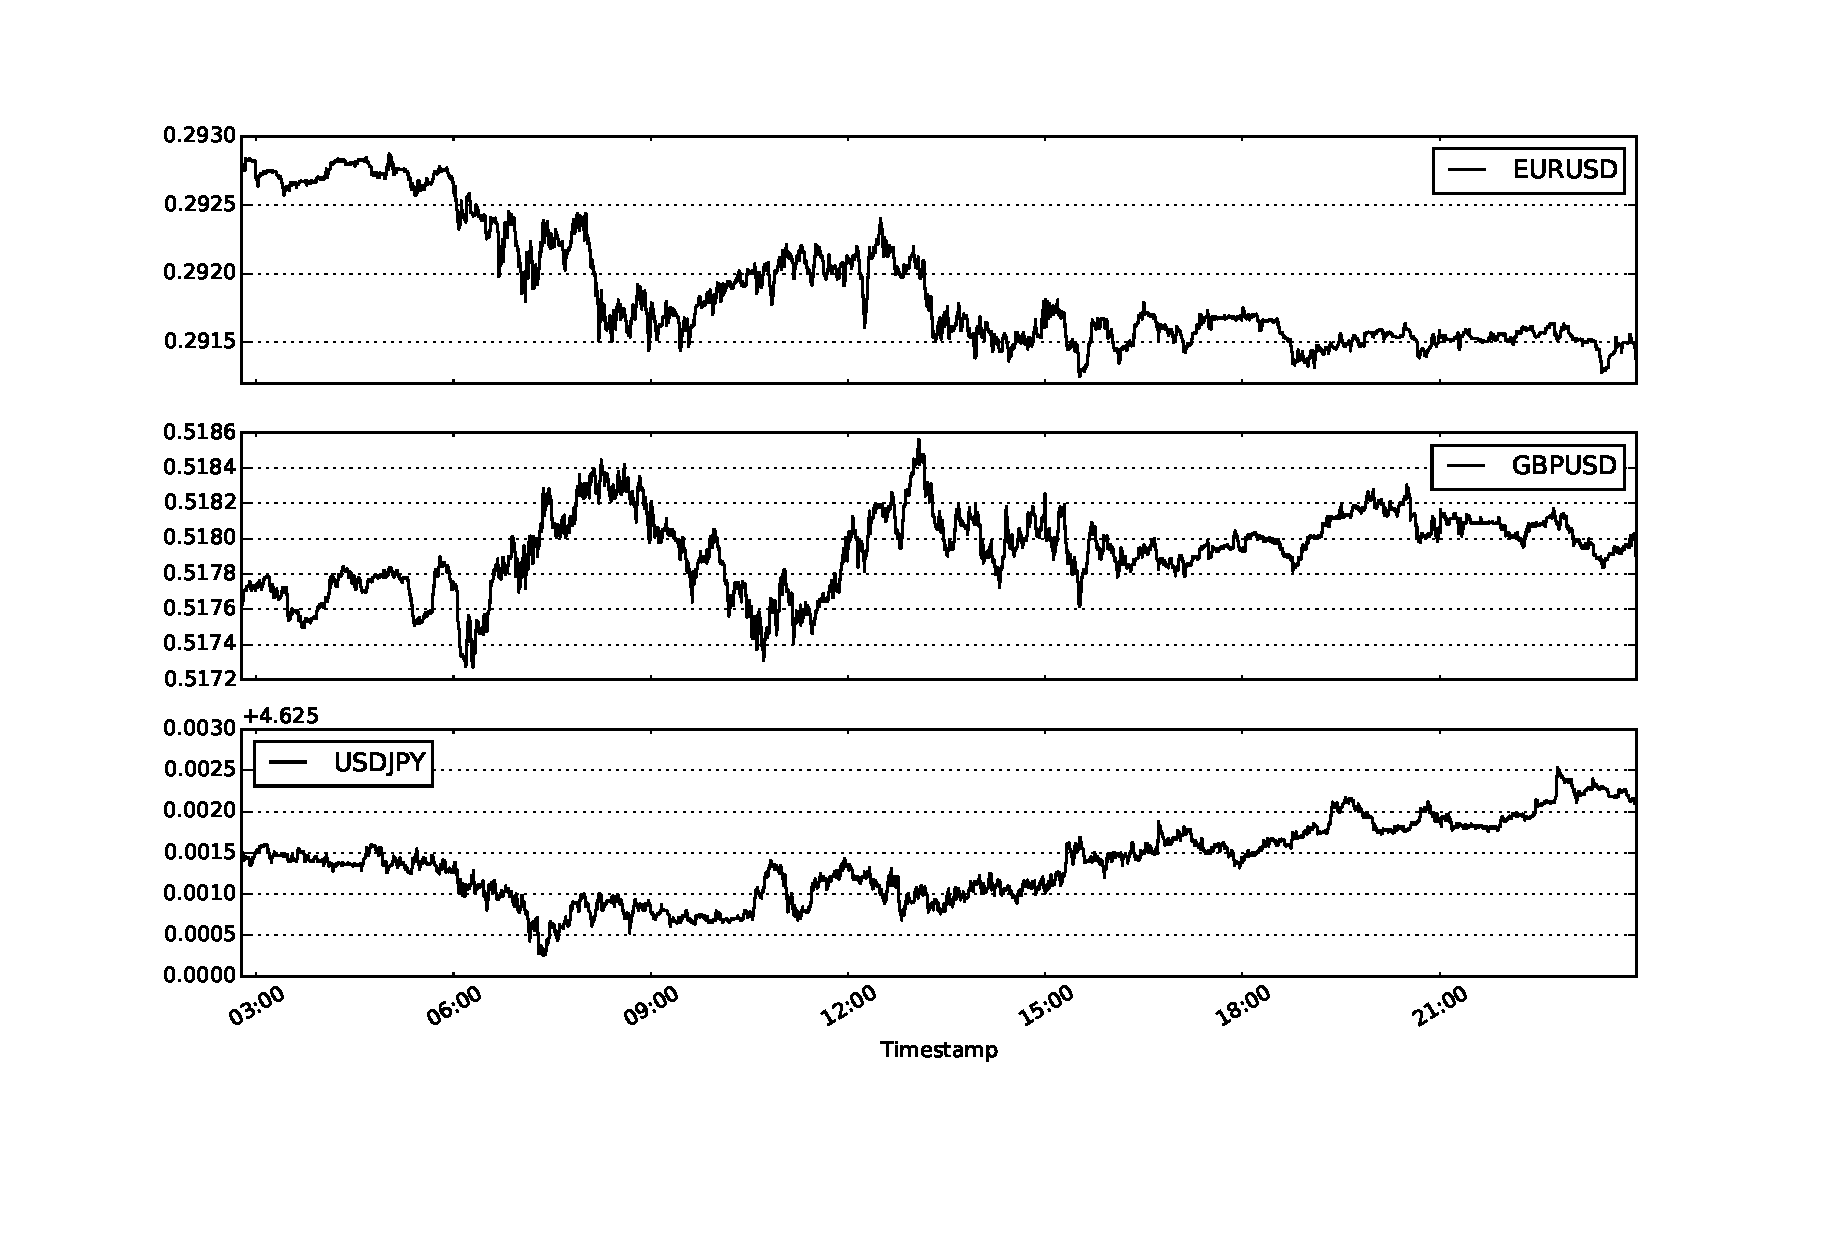
\includegraphics[width=0.4\textwidth]{forexdata}
  \caption{10 seconds frequency forex data for EURUSD, GBPUSD and USDJPY}
  \label{fig:forexdata}
\end{figure}

\begin{figure}[!ht]
  %\vspace{-0.8cm}
  \centering
  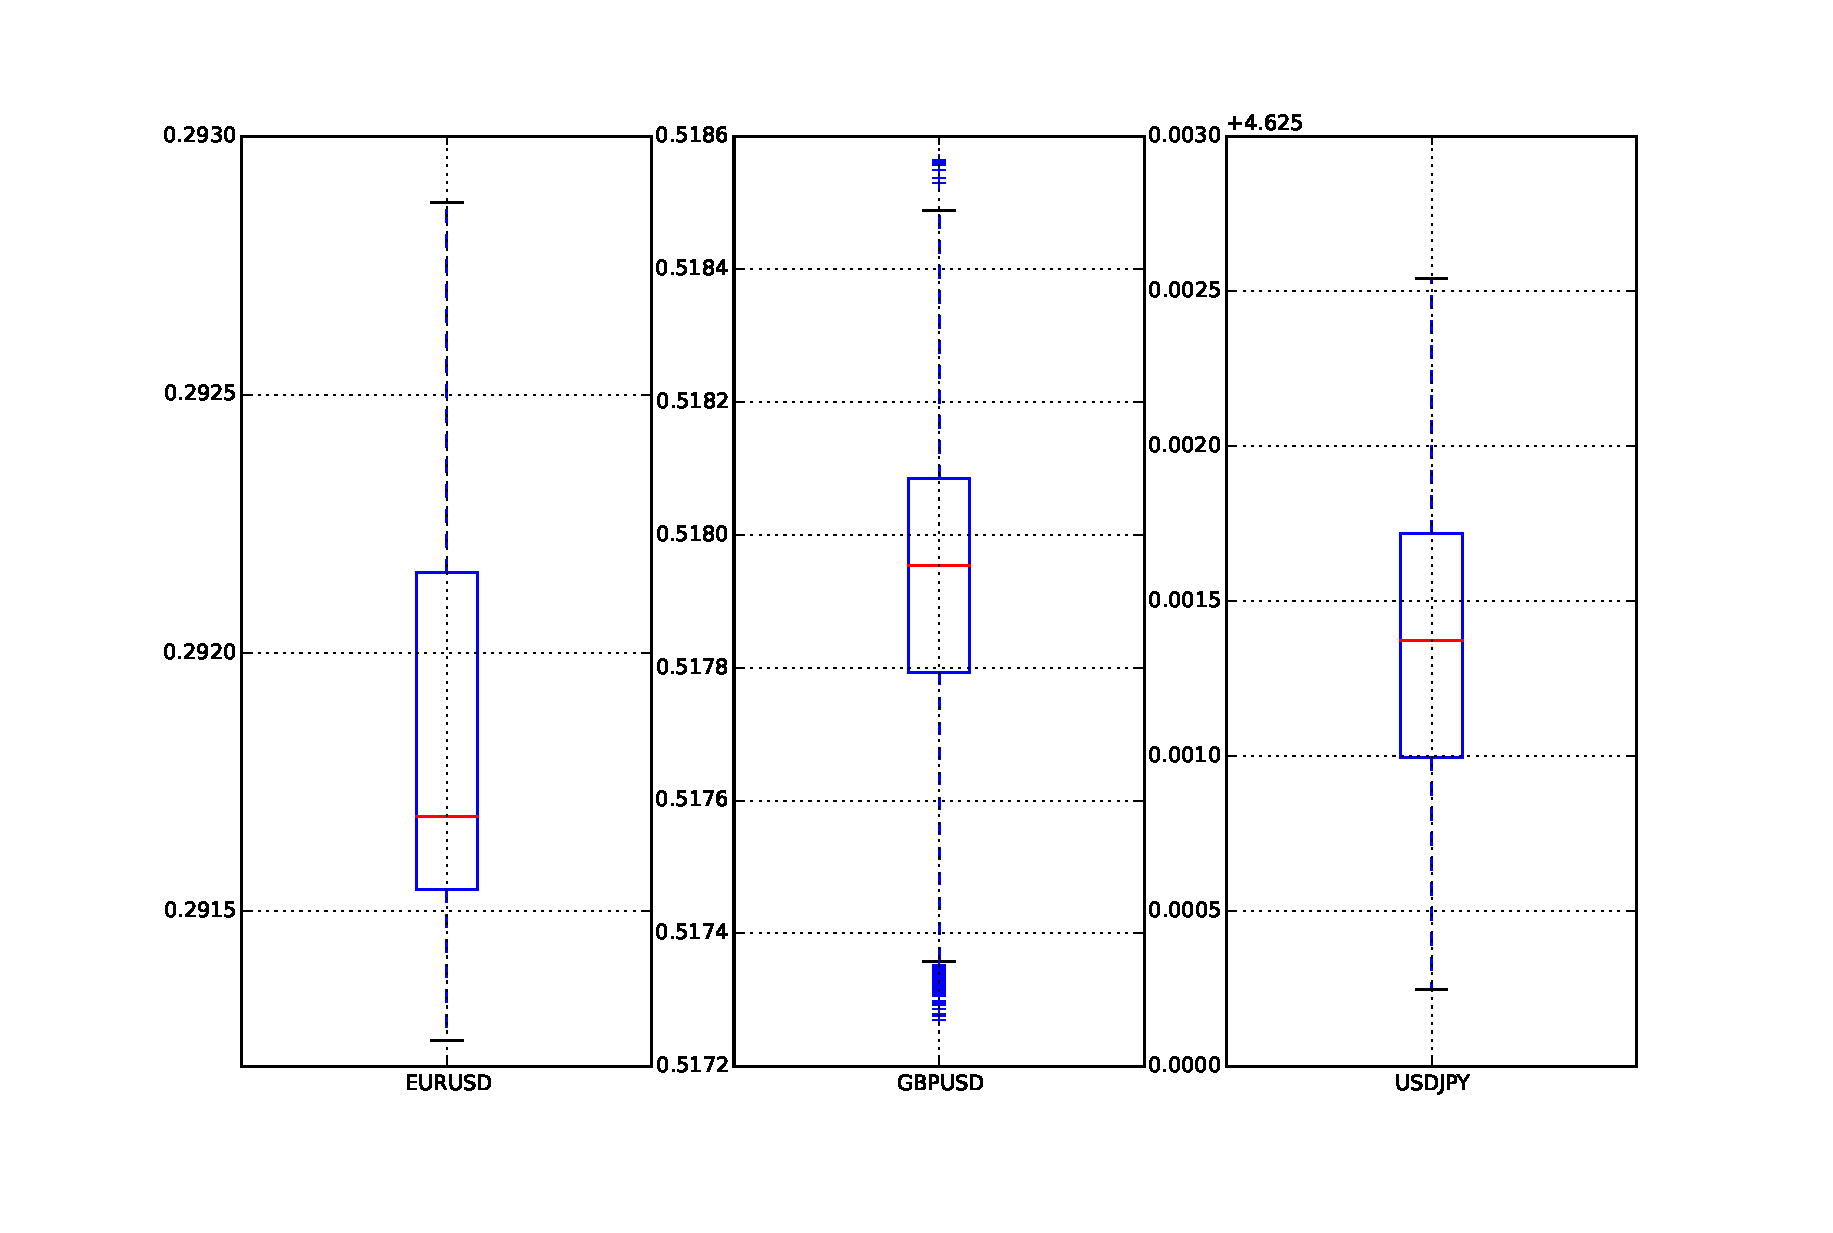
\includegraphics[width=0.4\textwidth]{distdata}
  \caption{Distribution of EURUSD, GBPUSD and USDJPY data}
  \label{fig:distdata}
\end{figure}


\begin{figure}[!ht]
  %\vspace{-0.8cm}
  \centering
  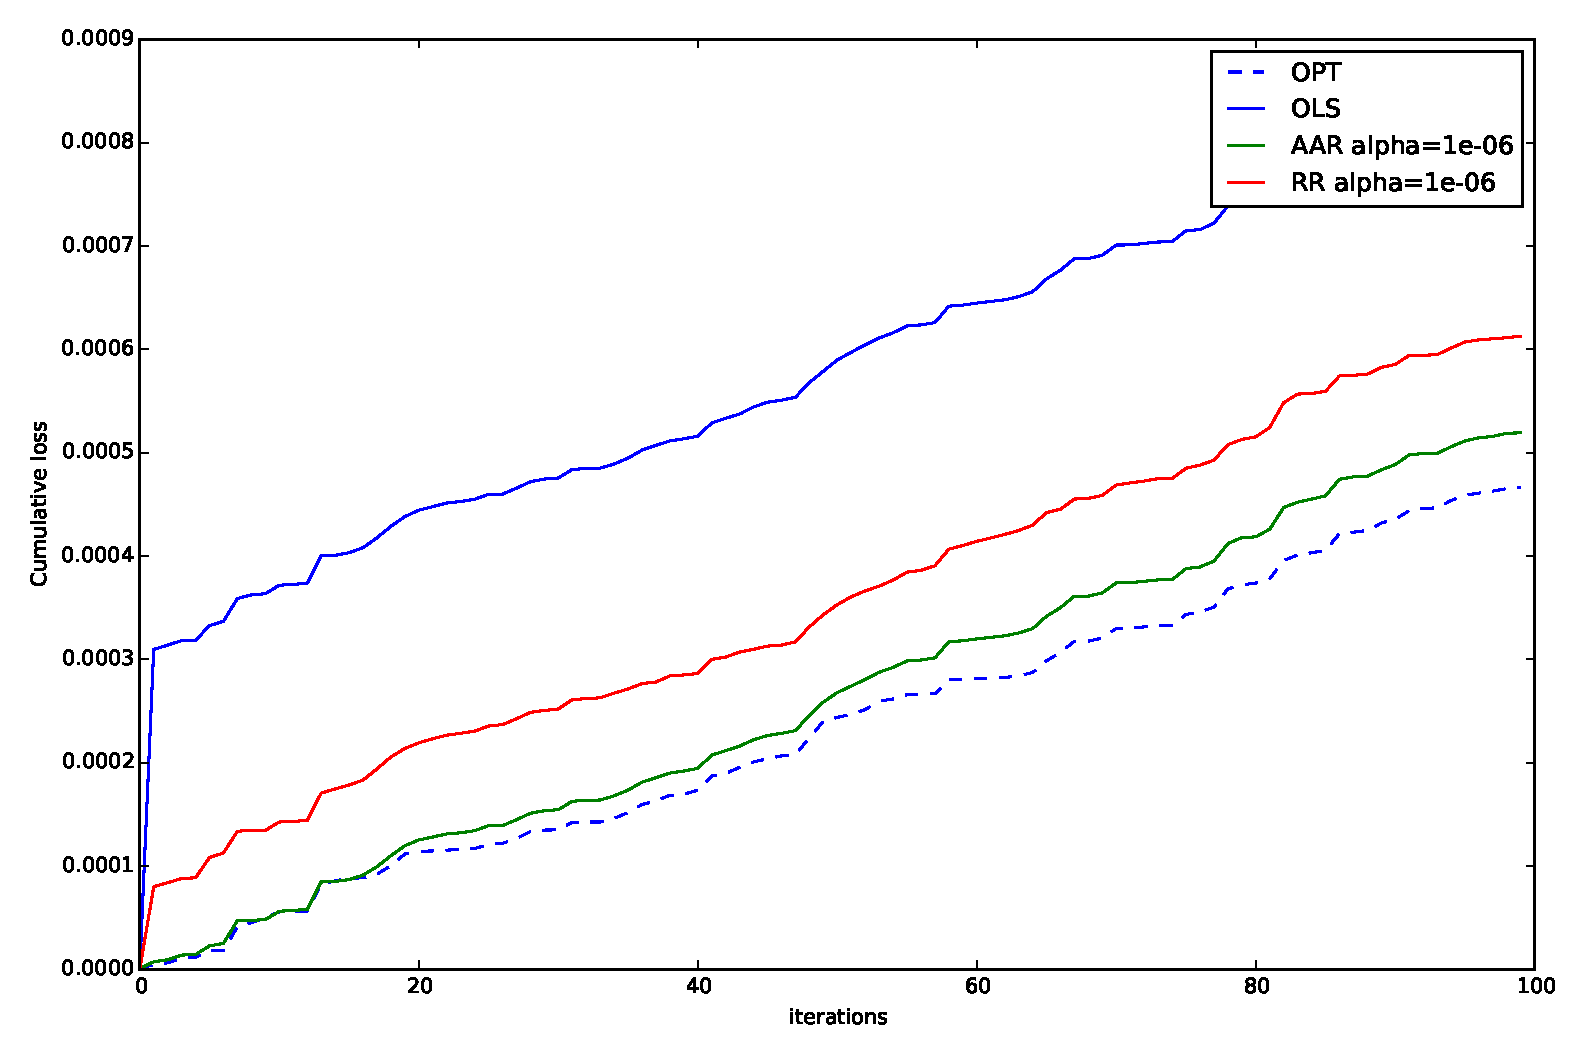
\includegraphics[width=0.4\textwidth]{onlinecomparison}
  \caption{Cumulative loss of AAR, RR and OLS solutions for VECM against its optimal algorithm}
  \label{fig:onlinecomparison}
\end{figure}


\begin{figure}[!ht]
  %\vspace{-0.8cm}
  \centering
  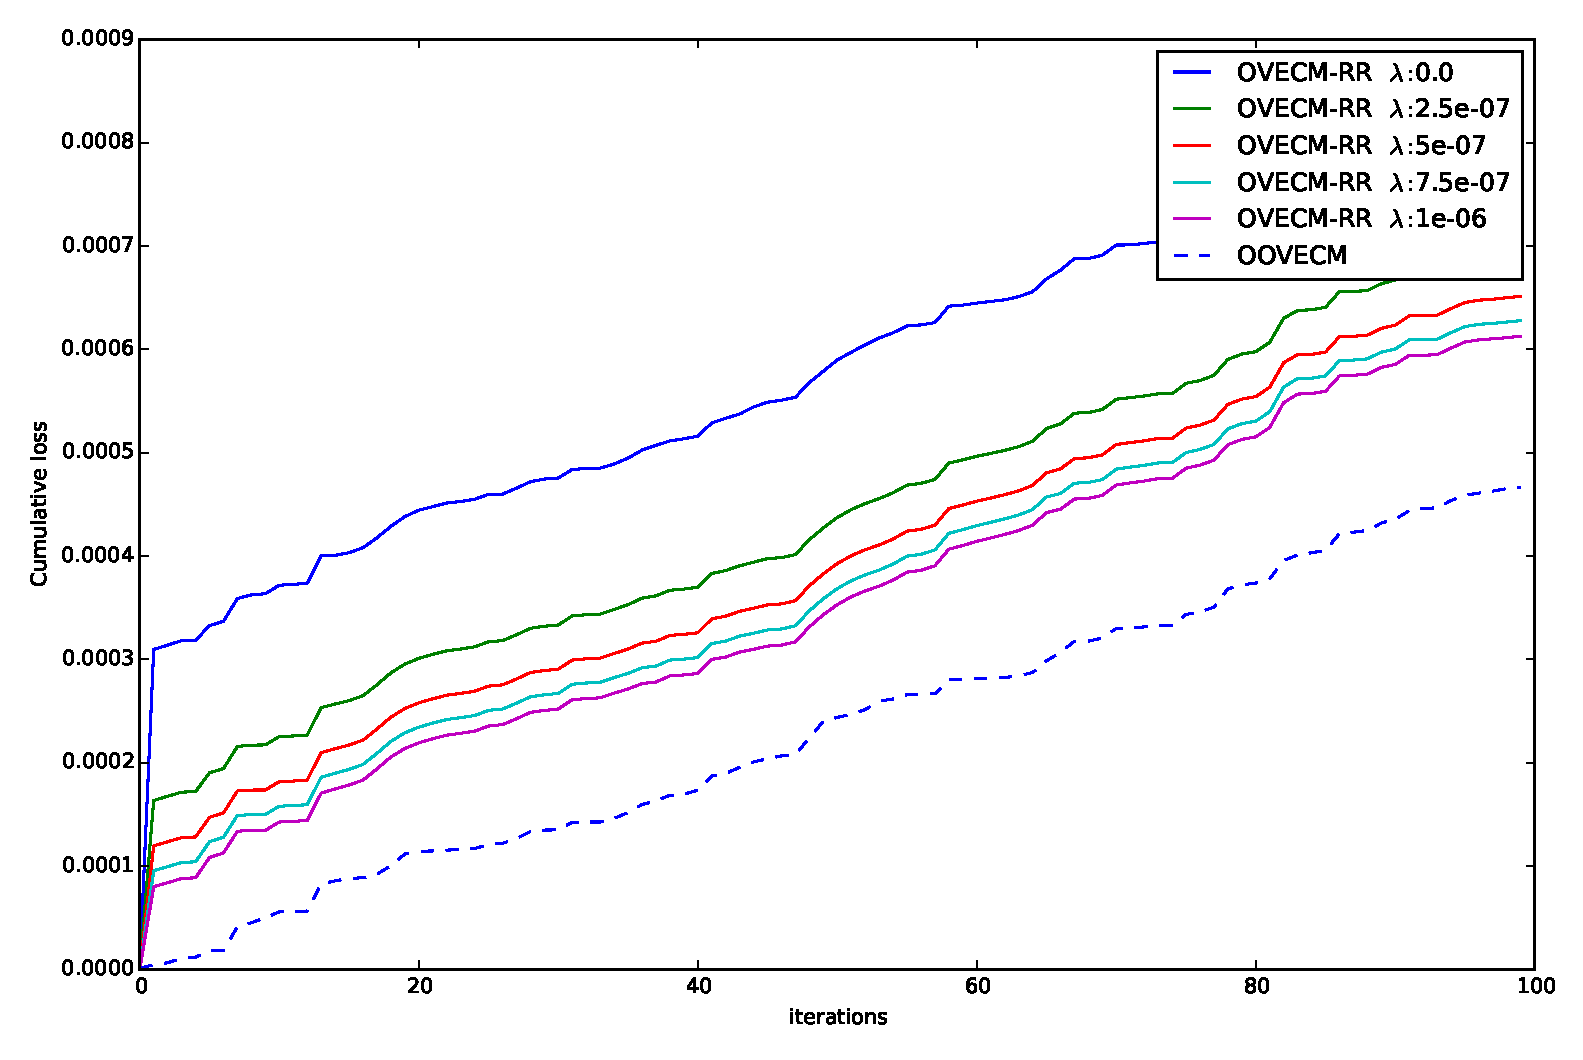
\includegraphics[width=0.4\textwidth]{RRcomparison}
  \caption{Cumulative loss RR VECM against its optimal algorithm using different $\lambda$ values}
  \label{fig:RRcomparison}
\end{figure}


\begin{figure}[!ht]
  %\vspace{-0.8cm}
  \centering
  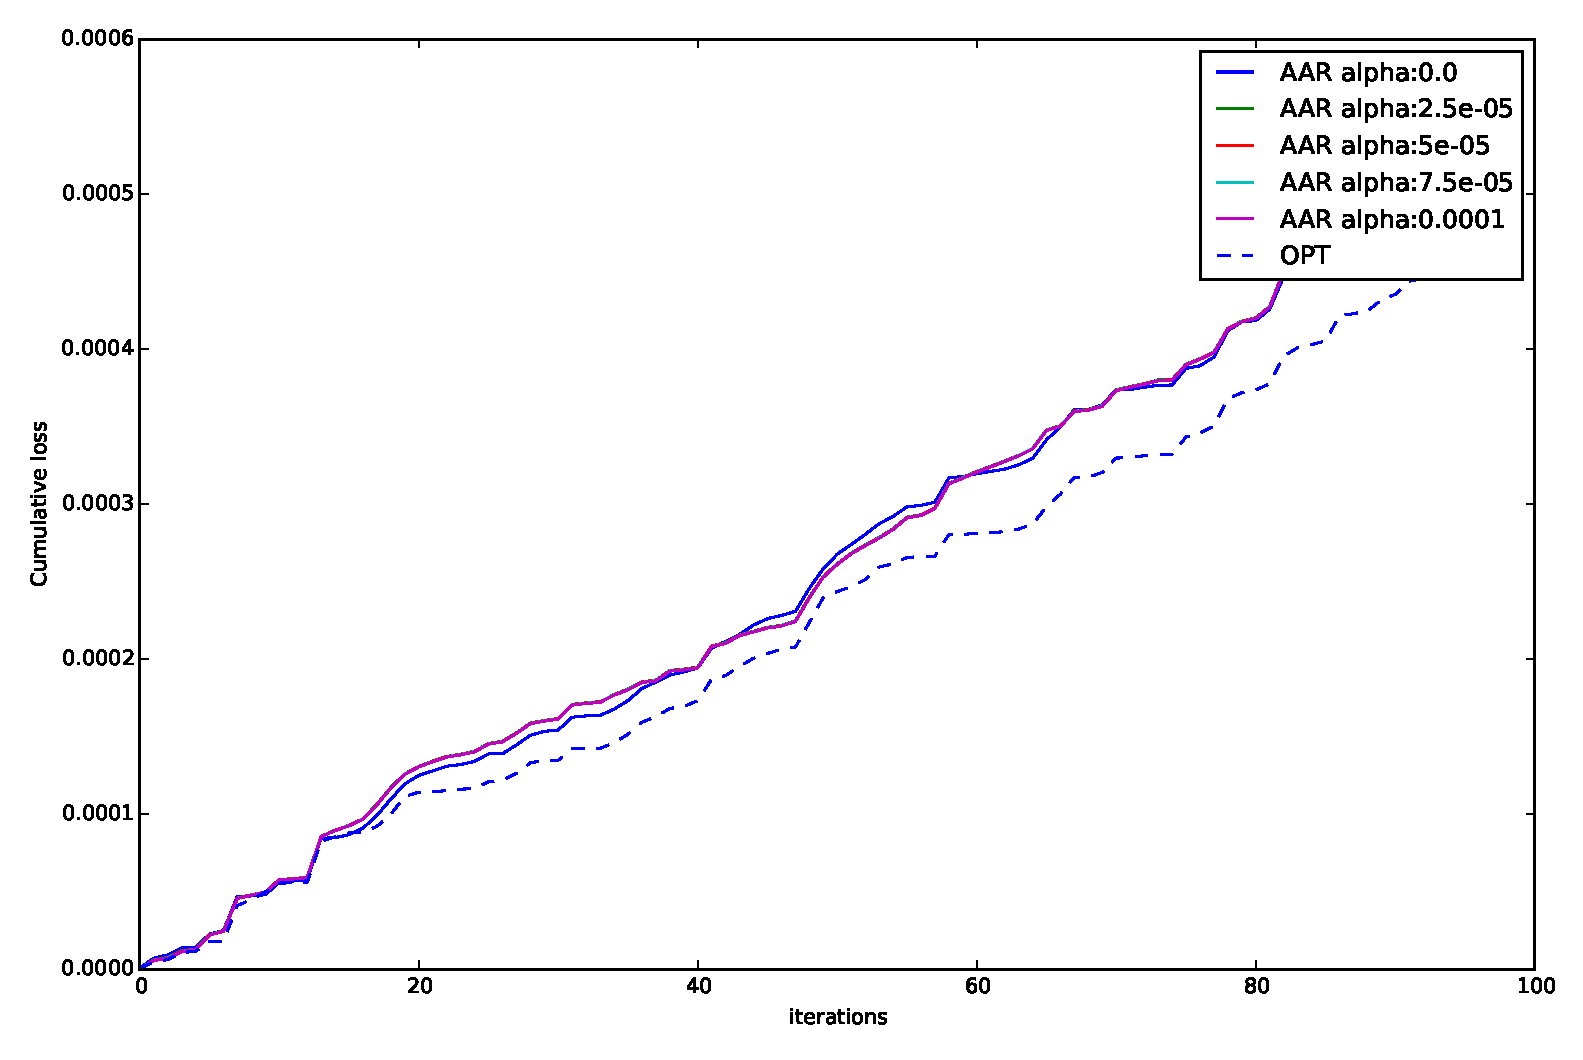
\includegraphics[width=0.4\textwidth]{AARcomparison}
  \caption{Cumulative loss AAR VECM against its optimal algorithm using different $\lambda$ values}
  \label{fig:AARcomparison}
\end{figure}

\section{Conclusions}
\label{sec:conclusions}
kk

\bibliographystyle{plain}       % APS-like style for physics

\bibliography{reference}   % name your BibTeX data base

\end{document}
% end of file template.tex

